
% Slideshow, written by Brent Baccala, for a lecture at Catholic University

\documentclass{beamer}
\usetheme{Madrid}

\title{Alternate techniques for solving systems of polynomial equations}
\author{Brent Baccala}
\institute{\tt cosine@freesoft.org}
\date{February 8, 2023}

\setbeamertemplate{footline}{}
\beamertemplatenavigationsymbolsempty

\usepackage{xcolor}
\usepackage{comment}
\usepackage{graphicx}

\usepackage{tabularx}

\begin{document}


\begin{frame}
\titlepage
\begin{block}{Abstract}
\tiny
While Buchberger's algorithm to construct Gr\"obner bases has justifiably been the subject of study and acclaim since its introduction in 1965, alternate strategies and algorithms exist to solve systems of polynomial equations.  Numerical techniques can be used to construct witness points, which are approximate solutions accurate enough that exact solutions can be recovered from them.  This talk will outline a basic technique for recovering exact solutions from witness points and describe two numerical algorithms used to construct witness points: the homotopy continuation method used by the Bertini software program, and the root finding algorithm used by the speaker to study differential equations.
\end{block}
\end{frame}

\begin{frame}
\frametitle{Part 1}
\begin{itemize}
\item START A RECORDER
\item give a simple example of reducing a polynomial mod an ideal using FLINT routine
\item is this a good idea?
\item illustrate the problem; it can be solved using Grobner bases
\item need to specify a monomial ordering: it matters in the multivariate case

\item solving systems of polynomial equations
\item two examples from Prof. Levin's talk: Lagrange multipliers and graph coloring
\item one is always a special case: linear algebra, matrix methods, LU decomposition
\item higher degree polynomials - Gr\"obner bases
\item demonstrate using two examples

\item performance problems with Buchberger's algorithm: the F4 and F5 algorithms
\begin{itemize}
   \item computing a Gr\"obner basis is NP-hard in general
   \item Faug\'ere's F5 algorithm
\end{itemize}
\end{itemize}
\end{frame}

\begin{frame}

\begin{exampleblock}{Learning a performance metric of Buchberger's algorithm

Jelena Mojsilovi\'c, Dylan Peifer, Sonja Petrovi\'c ({\tt arxiv.org}, 2021)
}
Many computer algebra systems offer generic algorithms for computing Gr\"obner bases
applicable to all kinds of input ideals. In the 1960s, Buchberger developed a groundbreaking
algorithm [Buchberger, 2006] to compute a Gr\"obner basis of any ideal, a problem that is
NP-hard in general. As it applies to any polynomial system, Buchberger's algorithm has a
doubly exponential runtime in the number of variables [Dube, 1990]. In the decades that followed,
several specialized algorithms have been used to improve runtime: Belt\'ran and Pardo
[2008, 2009.], Cox et al. [2007]. These algorithms form the cornerstone of the field of symbolic
computational nonlinear algebra.
\end{exampleblock}

\end{frame}

\begin{frame}
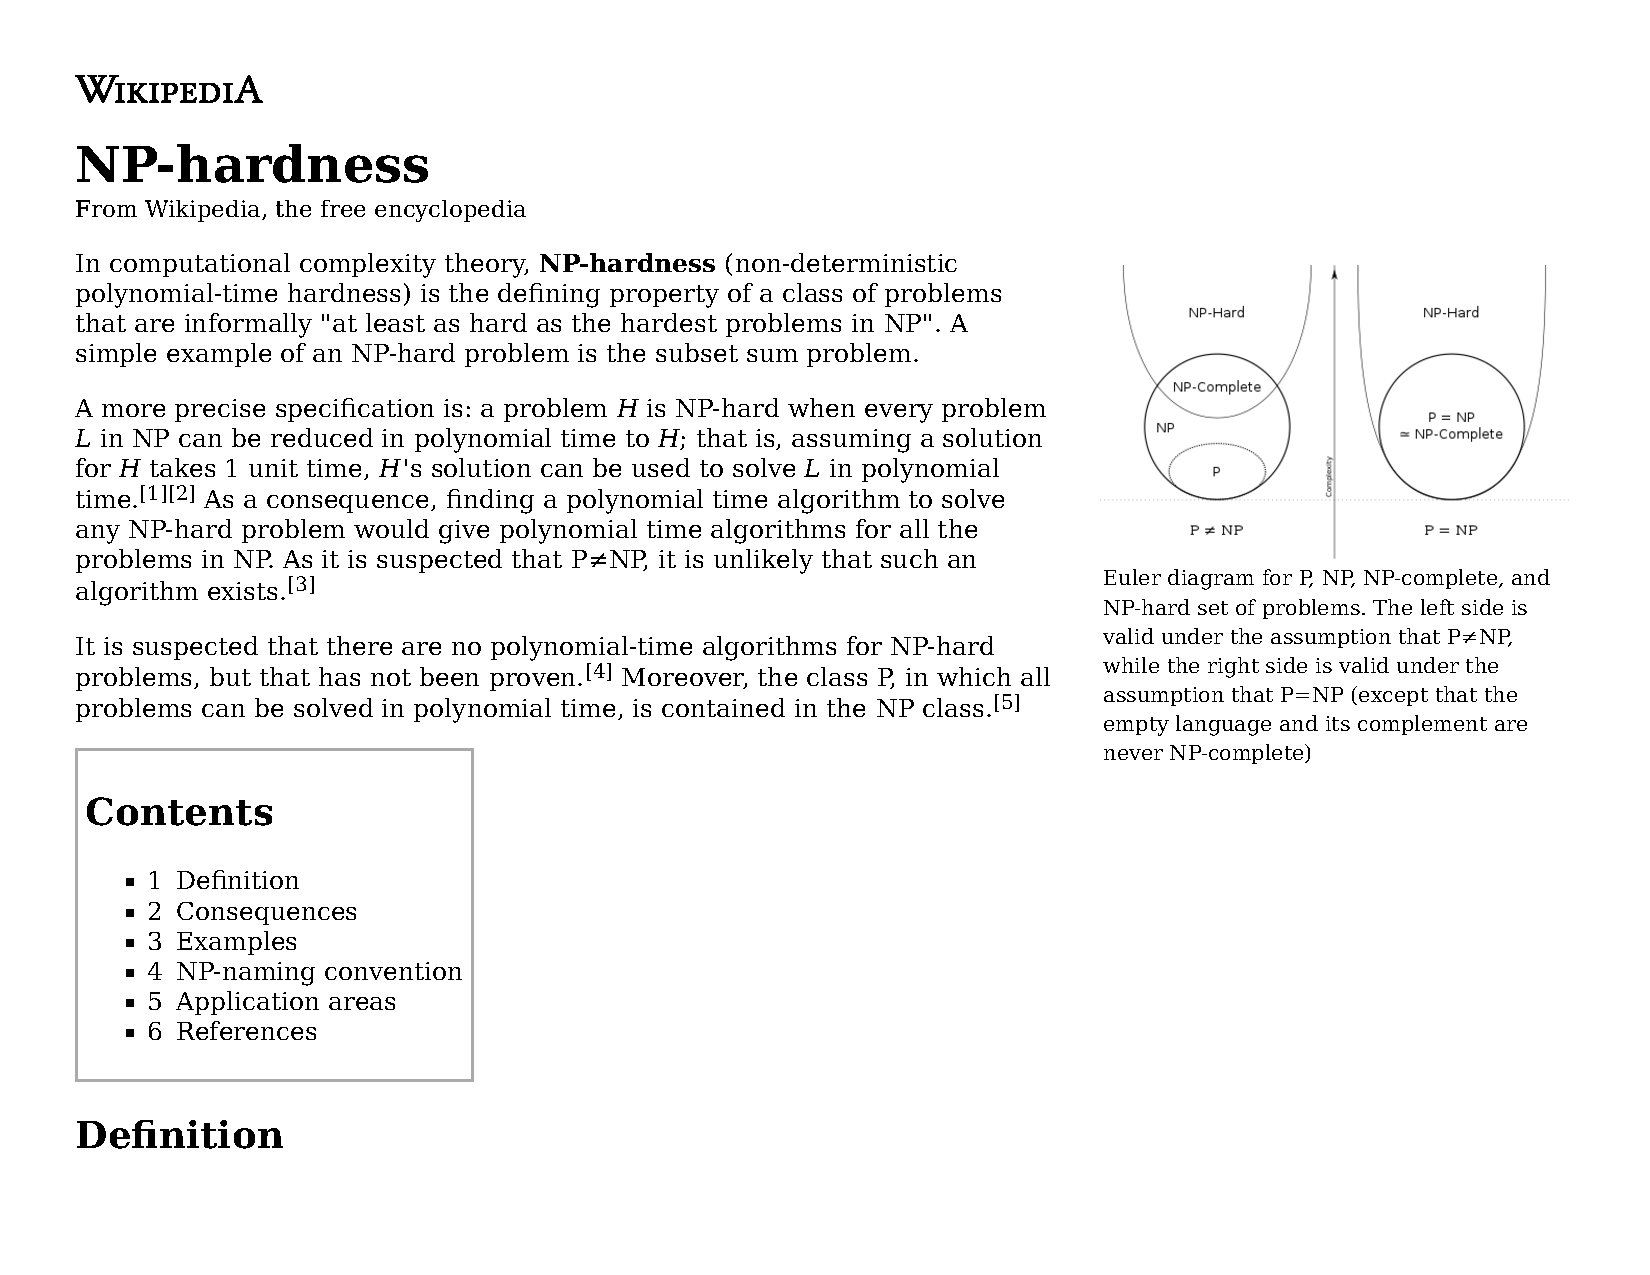
\includegraphics[width=\textwidth]{NP-hardness - Wikipedia.pdf}
\end{frame}

\begin{frame}

\begin{exampleblock}{Learning a performance metric of Buchberger's algorithm

Jelena Mojsilovi\'c, Dylan Peifer, Sonja Petrovi\'c ({\tt arxiv.org}, 2021)
}
Improvements on Buchberger's algorithm, such as Faug\'ere's famous F5 algorithm developed
in Faug\'ere et al. [1993], Faug\'ere et al. [2014], leverage the fact that the computation is
a generalization of Gaussian elimination. As such, these methods construct nontrivial
organizational techniques, such as cleverly organizing monomials into large matrices, to judiciously
perform Buchberger's key step: reduction of S-polynomials. Namely, the algorithm grows a
given generating set by adding nonzero remainders of S-polynomials upon division by the
current generating set; an S-polynomial is an element of the ideal created from a pair of
given polynomials. The correctness of Buchberger's algorithm does not depend on the order
in which such pairs, called S-pairs, are processed: one can simply create all pairs, store them
in a queue in arbitrary order, and process them linearly. On the other hand, the above
mentioned algorithms indicate – and by now this is part of the computational nonlinear algebra
folklore – one can improve the runtime by reorganizing the polynomials in the generating set
so as to process the S-pairs in different order.
%Standard strategies select pairs based on some
%minimality criterion, such as the degree of the least common multiple of the two leading terms
%or its position in the monomial order.
\end{exampleblock}

\end{frame}

\begin{frame}

\begin{exampleblock}{Learning a performance metric of Buchberger's algorithm

Jelena Mojsilovi\'c, Dylan Peifer, Sonja Petrovi\'c ({\tt arxiv.org}, 2021)
}
Within the paradigm of using
learning to improve algorithms that give the exact answer, Peifer et al. [2020] uses machine
learning to discover new S-pair selection strategies in Buchberger's algorithm which outperform
state-of-the-art human-designed heuristics by 20\% to 40\%. Their main contribution was
to express S-pair selection in Buchberger's algorithm as a reinforcement learning problem, i.e.
a game where the player or agent selects S-pairs and is rewarded for minimizing the overall
computational cost of the algorithm. Their measure of computational cost was the number
of polynomial additions performed, which is a hardware- independent number that indicates
how hard the basis was to compute.
\end{exampleblock}

\end{frame}

\begin{frame}

\begin{exampleblock}{Learning a performance metric of Buchberger's algorithm

Jelena Mojsilovi\'c, Dylan Peifer, Sonja Petrovi\'c ({\tt arxiv.org}, 2021)
}
A key part of many reinforcement learning techniques
is a value model which learns to predict future reward...
such a model would predict the number of future polynomial
additions before the Gr\"obner basis computation is complete. The goal of this manuscript is
to learn a version of this value function in the supervised learning setting
\end{exampleblock}

\begin{exampleblock}{}
JM is a PhD student at Purdue University. SP is with Illinois Tech's Applied Math Department, and
partially supported by the Simons Foundation Collaboration Grant for Mathematicians 854770. At the time
of the first version of this manuscript, JM was an Applied Math undergraduate researcher at Illinois Tech and
DP was a Mathematics PhD student at Cornel
\end{exampleblock}

\end{frame}

\begin{frame}
\frametitle{Systems of linear polynomials (1 is always a special case)}

%% LU decomposition
\includegraphics[width=\textwidth, page=13]{LU decomposition - Wikipedia.pdf}
\end{frame}

\begin{frame}
\begin{itemize}
\item alternatives: numerical techniques
\item witness points: approximate solutions accurate enough to find exact solutions
\item LLL algorithm

\item Andrew Sommese - Notre Dame

Daniel J. Bates, Jonathan D. Hauenstein, Timothy M. McCoy, Chris Peterson \& Andrew J. Sommese (2013)
Recovering Exact Results from Inexact Numerical Data in Algebraic Geometry,
Experimental Mathematics, 22:1, 38-50, DOI: 10.1080/10586458.2013.737640

\item "exactness recovery algorithms"
\item https://en.wikipedia.org/wiki/Lenstra%E2%80%93Lenstra%E2%80%93Lov%C3%A1sz_lattice_basis_reduction_algorithm

\item Newton's method
     {\tt https://en.wikipedia.org/wiki/File:NewtonIteration\_Ani.gif}

\item Bertini's homotopy continuation method
\item {\tt https://en.wikipedia.org/wiki/Homotopy}
\end{itemize}
\end{frame}

\begin{frame}
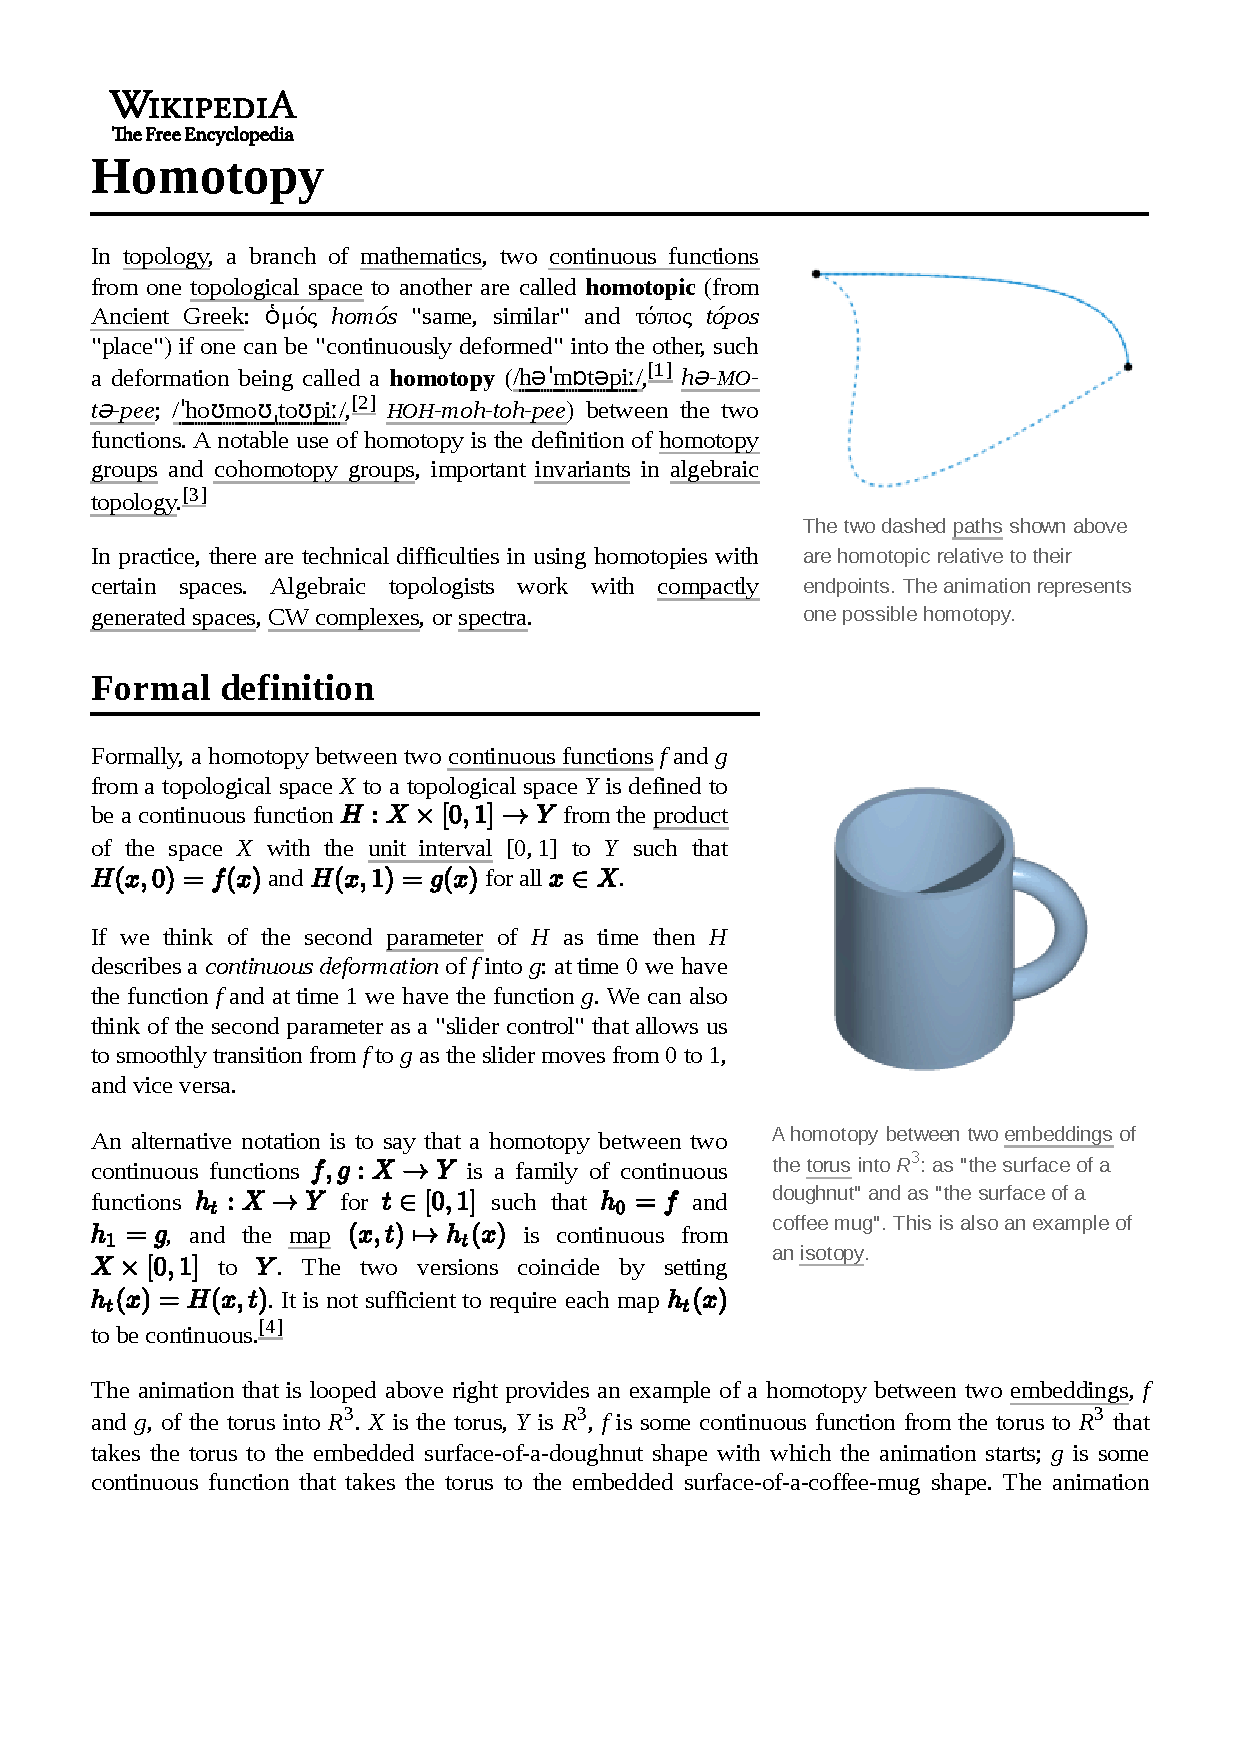
\includegraphics[width=\textwidth]{Homotopy.pdf}
\end{frame}

\begin{frame}
\frametitle{Part 2}

\begin{itemize}
\item ASIDE: Rosenfeld-Grobner in differential algebra
\item my code: scipy's levenberg-marquet algorithm
\item my algorithm for fast evaluation of polynomials and Jacobians using sparse matrices
\item optimization: use shared memory to run computations in parallel
\item potential scipy optimization for parallel QR decomposition
\item potential scipy optimization for superscalar sparse multiplication
     types of matrix storage layouts: dense, sparse (COO, CSC, CSR, DOK)
%     csr_matvec in ~/src/scipy/scipy/sparse/sparsetools/csr.h

\item example: the f(x+r) solutions
\item show several examples, lattice reduction by hand, and demonstrate that it's a dot product
\item why it doesn't solve Schrodinger globally
\item using Kovacic's algorithm to determine that it's non-elementary
\item Mathematica says it's related to the Bessel functions
\item show how
\end{itemize}
\end{frame}

\begin{frame}[fragile]
\frametitle{Hydrogen ansatz 5}
\begin{semiverbatim}
\tiny
\textcolor{blue}{sage:} load('helium.sage')
\textcolor{blue}{sage:} prep_hydrogen(5)
\textcolor{blue}{sage:} multi_init()
\textcolor{blue}{sage:} multi_expand()
\textcolor{blue}{sage:} random_numerical(homogenize=1)

...
6.169694306802097e-32                0.12 sec


(E, 4.6673330021180737e-20)
(b0, 1.0)
(b1, 0.464918758265008)
(b2, 4.9956745914527553e-20)
(b3, 0.5179110625786596)
(b4, -1.6316396076549894e-19)
(b5, 0.7180659297529489)
(b6, 8.416841906183793e-20)
(d0, -1.2625718788062294e-26)
(d1, 1.0)
(m0, -1.0)
(m1, 1.0711161751949155e-20)
(n0, -1.0)
(n1, -6.556316253156553e-20)
\end{semiverbatim}
\vskip 0pt plus 100fill
\end{frame}

\begin{frame}[fragile]
\frametitle{scipy's sparse CSR matrix vector multiplication routine}
%% ~/src/scipy/scipy/sparse/sparsetools/csr.h
\begin{semiverbatim}
\tiny
/* Compute Y += A*X for CSR matrix A and dense vectors X,Y
 *
 * Input Arguments:
 *   I  n_row         - number of rows in A
 *   I  n_col         - number of columns in A
 *   I  Ap[n_row+1]   - row pointer
 *   I  Aj[nnz(A)]    - column indices
 *   T  Ax[nnz(A)]    - nonzeros
 *   T  Xx[n_col]     - input vector
 *
 * Output Arguments:
 *   T  Yx[n_row]     - output vector
 *
 * Note:
 *   Output array Yx must be preallocated
 *
 *   Complexity: Linear.  Specifically O(nnz(A) + n_row)
 */
template <class I, class T>
void csr_matvec(const I n_row, const I n_col, const I Ap[],
                const I Aj[],  const T Ax[],  const T Xx[], T Yx[])
\{
    for(I i = 0; i < n_row; i++)\{
        T sum = Yx[i];
        for(I jj = Ap[i]; jj < Ap[i+1]; jj++)\{
            sum += Ax[jj] * Xx[Aj[jj]];
        \}
        Yx[i] = sum;
    \}
\}

\end{semiverbatim}
\vskip 0pt plus 100fill
\end{frame}

\begin{frame}[fragile]
\frametitle{gcc's assembly code for the inner loop ({\tt -mavx2 -O3})}
%% cat sparse1.c
%% objdump -dwr --no-show-raw-insn sparse1.o | sed 's/#[^<]*<[^>]*>//' | grep '^ *[0-9a-f]*:' | column -t
\begin{semiverbatim}
\tiny
double sum;

const int Aj[4];
const double Ax[4];
const double Xx[4];

void vecmult(void)
\{
    for(int jj = 0; jj < 4; jj++) \{
        sum += Ax[jj] * Xx[Aj[jj]];
    \}
\}

0:   endbr64
4:   movslq       0x0(%rip),%rdx             7:   R_X86_64_PC32  Aj-0x4
b:   lea          0x0(%rip),%rax             e:   R_X86_64_PC32  Xx-0x4
12:  vmovsd       0x0(%rip),%xmm1            16:  R_X86_64_PC32  sum-0x4
1a:  vmovsd       0x0(%rip),%xmm2            1e:  R_X86_64_PC32  Ax+0x4
22:  vmovsd       0x0(%rip),%xmm3            26:  R_X86_64_PC32  Ax+0xc
2a:  vmovsd       0x0(%rip),%xmm4            2e:  R_X86_64_PC32  Ax+0x14
32:  vmovsd       (%rax,%rdx,8),%xmm0
37:  movslq       0x0(%rip),%rdx             3a:  R_X86_64_PC32  Aj
3e:  vfmadd132sd  0x0(%rip),%xmm1,%xmm0      43:  R_X86_64_PC32  Ax-0x4
47:  vfmadd231sd  (%rax,%rdx,8),%xmm2,%xmm0
4d:  movslq       0x0(%rip),%rdx             50:  R_X86_64_PC32  Aj+0x4
54:  vfmadd231sd  (%rax,%rdx,8),%xmm3,%xmm0
5a:  movslq       0x0(%rip),%rdx             5d:  R_X86_64_PC32  Aj+0x8
61:  vfmadd231sd  (%rax,%rdx,8),%xmm4,%xmm0
67:  vmovsd       %xmm0,0x0(%rip)            6b:  R_X86_64_PC32  sum-0x4
6f:  retq

\end{semiverbatim}
\vskip 0pt plus 100fill
\end{frame}

\begin{frame}[fragile]
\frametitle{Improvement: using an array of accumulators}
%% cat sparse4.c
%% objdump -dwr --no-show-raw-insn sparse4.o | sed 's/#[^<]*<[^>]*>//' | grep '^ *[0-9a-f]*:' | column -t
\begin{semiverbatim}
\scriptsize

double tmp1[4] __attribute__((aligned(32)));
double tmp2[4] __attribute__((aligned(32)));
double tmp3[4] __attribute__((aligned(32)));

void vecmult(void)
\{
    for (int i=0; i<4; i++) \{
        tmp3[i] += tmp1[i] * tmp2[i];
    \}
\}

0:   endbr64
4:   vmovapd     0x0(%rip),%ymm1        8:   R_X86_64_PC32  tmp1-0x4
c:   vmulpd      0x0(%rip),%ymm1,%ymm0  10:  R_X86_64_PC32  tmp2-0x4
14:  vaddpd      0x0(%rip),%ymm0,%ymm0  18:  R_X86_64_PC32  tmp3-0x4
1c:  vmovapd     %ymm0,0x0(%rip)        20:  R_X86_64_PC32  tmp3-0x4
24:  vzeroupper
27:  retq

\end{semiverbatim}
\vskip 0pt plus 100fill
\end{frame}

\end{document}
